% =============================================================================
% Lecture 01: Introduction to Forecasting
% BSAD 8310: Business Forecasting
% University of Nebraska at Omaha
% =============================================================================

\documentclass[aspectratio=169, 11pt]{beamer}

% =============================================================================
% header.tex — BSAD 8310: Business Forecasting
% University of Nebraska at Omaha
% Beamer theme: UNO-branded, clean, professional
% =============================================================================

% ----------------------------- BEAMER THEME ----------------------------------
\usetheme{default}
\useinnertheme{rectangles}

% ----------------------------- UNO COLOR PALETTE -----------------------------
\definecolor{unoblue}{HTML}{005CA9}
\definecolor{unored}{HTML}{E41C38}
\definecolor{unogray}{HTML}{525252}
\definecolor{unogreen}{HTML}{15803d}
\definecolor{unolightblue}{HTML}{E8F0FA}
\definecolor{unolightred}{HTML}{FDECEA}
\definecolor{unolightgreen}{HTML}{F0FAF4}
\definecolor{unowhite}{HTML}{FFFFFF}

% Apply UNO colors to Beamer structure
\setbeamercolor{structure}{fg=unoblue}
\setbeamercolor{palette primary}{bg=unoblue, fg=white}
\setbeamercolor{palette secondary}{bg=unoblue!80!black, fg=white}
\setbeamercolor{palette tertiary}{bg=unoblue!60!black, fg=white}
\setbeamercolor{frametitle}{bg=unoblue, fg=white}
\setbeamercolor{frametitle right}{bg=unoblue!80!black}
\setbeamercolor{title}{fg=unoblue}
\setbeamercolor{subtitle}{fg=unogray}
\setbeamercolor{author in head/foot}{bg=unoblue, fg=white}
\setbeamercolor{title in head/foot}{bg=unoblue!80, fg=white}
\setbeamercolor{date in head/foot}{bg=unoblue!60, fg=white}
\setbeamercolor{page number in head/foot}{bg=unoblue!60, fg=white}
\setbeamercolor{block title}{bg=unoblue, fg=white}
\setbeamercolor{block body}{bg=unolightblue}
\setbeamercolor{block title alerted}{bg=unored, fg=white}
\setbeamercolor{block body alerted}{bg=unolightred}
\setbeamercolor{block title example}{bg=unogreen, fg=white}
\setbeamercolor{block body example}{bg=unolightgreen}
\setbeamercolor{itemize item}{fg=unoblue}
\setbeamercolor{itemize subitem}{fg=unored}
\setbeamercolor{enumerate item}{fg=unoblue}
\setbeamercolor{enumerate subitem}{fg=unored}
\setbeamercolor{alerted text}{fg=unored}

% ----------------------------- FONTS -----------------------------------------
\usefonttheme{professionalfonts}
\usefonttheme[onlymath]{serif}       % serif math; sans-serif text
\setbeamerfont{frametitle}{size=\large, series=\bfseries}
\setbeamerfont{title}{size=\LARGE, series=\bfseries}
\setbeamerfont{subtitle}{size=\large}
\setbeamerfont{block title}{size=\normalsize, series=\bfseries}
\setbeamerfont{footline}{size=\tiny}

% ----------------------------- LAYOUT ----------------------------------------
\setbeamersize{text margin left=0.5cm, text margin right=0.5cm}
\setbeamertemplate{navigation symbols}{}   % remove navigation buttons
\setbeamertemplate{itemize items}[circle]
\setbeamertemplate{enumerate items}[default]

% Custom footline: [Course] [Title] [Page/Total]
\setbeamertemplate{footline}{%
  \leavevmode%
  \hbox{%
    \begin{beamercolorbox}[wd=.33\paperwidth, ht=2.5ex, dp=1ex, left, leftskip=4pt]
      {author in head/foot}%
      \usebeamerfont{author in head/foot}\insertshortauthor
    \end{beamercolorbox}%
    \begin{beamercolorbox}[wd=.34\paperwidth, ht=2.5ex, dp=1ex, center]
      {title in head/foot}%
      \usebeamerfont{title in head/foot}\insertshorttitle
    \end{beamercolorbox}%
    \begin{beamercolorbox}[wd=.33\paperwidth, ht=2.5ex, dp=1ex, right, rightskip=4pt]
      {date in head/foot}%
      \usebeamerfont{date in head/foot}%
      \insertframenumber{} / \inserttotalframenumber
    \end{beamercolorbox}%
  }%
  \vskip0pt%
}

% Frametitle with thin accent line
\setbeamertemplate{frametitle}{%
  \vskip0.1cm
  \insertframetitle
  \vskip0.05cm
  \color{unored}\rule{\textwidth}{0.5pt}
}

% Title page
\setbeamertemplate{title page}{%
  \vfill
  \begin{center}
    {\color{unoblue}\rule{\textwidth}{2pt}}\\[0.3cm]
    {\usebeamerfont{title}\usebeamercolor[fg]{title}\inserttitle}\\[0.2cm]
    {\usebeamerfont{subtitle}\usebeamercolor[fg]{subtitle}\insertsubtitle}\\[0.3cm]
    {\color{unored}\rule{\textwidth}{0.5pt}}\\[0.4cm]
    {\small\insertauthor}\\[0.1cm]
    {\small\insertinstitute}\\[0.1cm]
    {\small\insertdate}
  \end{center}
  \vfill
}

% ----------------------------- PACKAGES --------------------------------------

% Math
\usepackage{amsmath}
\usepackage{amssymb}
\usepackage{mathtools}
\usepackage{bm}                    % bold math symbols

% Graphics & color
\usepackage{graphicx}
\usepackage{xcolor}
\usepackage{tikz}
\usetikzlibrary{arrows.meta, positioning, shapes, fit, backgrounds, calc}
\usepackage{pgfplots}
\pgfplotsset{compat=1.18}

% Tables
\usepackage{booktabs}
\usepackage{array}
\usepackage{multirow}
\usepackage{tabularx}

% Typography
\usepackage{microtype}
\usepackage{url}
\usepackage{hyperref}
\hypersetup{colorlinks=true, linkcolor=unoblue, urlcolor=unoblue, citecolor=unogray}

% Code listings (no shell-escape required)
\usepackage{listings}
\lstset{
  language=Python,
  basicstyle=\ttfamily\footnotesize,
  keywordstyle=\color{unoblue}\bfseries,
  stringstyle=\color{unogreen},
  commentstyle=\color{unogray}\itshape,
  numberstyle=\tiny\color{unogray},
  breaklines=true,
  showstringspaces=false,
  frame=single,
  rulecolor=\color{unogray!40},
  backgroundcolor=\color{unogray!5},
  xleftmargin=0.5em,
  xrightmargin=0.5em,
}

% Bibliography
\usepackage[backend=bibtex, style=authoryear, maxcitenames=2]{biblatex}
\addbibresource{../Bibliography_base.bib}

% Colored text helpers
\usepackage{tcolorbox}
\tcbuselibrary{skins, breakable, listingsutf8}

% ----------------------------- CUSTOM ENVIRONMENTS ---------------------------

% keybox: UNO-blue background — for key results, formulas, takeaways
\newtcolorbox{keybox}{
  enhanced,
  colback=unoblue,
  colframe=unoblue!80!black,
  coltitle=white,
  coltext=white,
  fonttitle=\bfseries,
  boxrule=0pt,
  arc=3pt,
  left=4pt, right=4pt, top=3pt, bottom=3pt,
}

% definitionbox: blue left-rule with title — for formal definitions
\newtcolorbox{definitionbox}[1]{
  enhanced,
  title={#1},
  colback=unolightblue,
  colframe=unoblue,
  coltitle=unoblue,
  fonttitle=\bfseries,
  boxrule=0pt,
  leftrule=3pt,
  arc=0pt,
  left=4pt, right=4pt, top=3pt, bottom=3pt,
}

% warningbox: red-accent — for pitfalls, assumption violations, common errors
\newtcolorbox{warningbox}{
  enhanced,
  colback=unolightred,
  colframe=unored,
  coltitle=white,
  fonttitle=\bfseries,
  boxrule=0pt,
  leftrule=3pt,
  arc=0pt,
  left=4pt, right=4pt, top=3pt, bottom=3pt,
}

% examplebox: green-accent with title — for worked examples, business applications
\newtcolorbox{examplebox}[1]{
  enhanced,
  title={#1},
  colback=unolightgreen,
  colframe=unogreen,
  coltitle=unogreen,
  fonttitle=\bfseries,
  boxrule=0pt,
  leftrule=3pt,
  arc=0pt,
  left=4pt, right=4pt, top=3pt, bottom=3pt,
}

% ----------------------------- MATH SHORTCUTS --------------------------------
\newcommand{\E}{\mathbb{E}}
\newcommand{\Var}{\operatorname{Var}}
\newcommand{\Cov}{\operatorname{Cov}}
\newcommand{\Corr}{\operatorname{Corr}}
\newcommand{\MSE}{\operatorname{MSE}}
\newcommand{\RMSE}{\operatorname{RMSE}}
\newcommand{\MAE}{\operatorname{MAE}}
\newcommand{\MASE}{\operatorname{MASE}}
\newcommand{\yhat}{\hat{y}}
\newcommand{\bhat}{\hat{\beta}}
\newcommand{\eps}{\varepsilon}
\newcommand{\given}{\,|\,}

% ----------------------------- SLIDE HELPERS ---------------------------------
% Section title slide (call at start of each section)
\newcommand{\sectionslide}[2]{%
  \begin{frame}
    \vfill
    \begin{center}
      {\color{unoblue}\rule{0.6\textwidth}{2pt}}\\[0.4cm]
      {\Large\bfseries\color{unoblue} #1}\\[0.2cm]
      {\normalsize\color{unogray} #2}\\[0.4cm]
      {\color{unored}\rule{0.6\textwidth}{1pt}}
    \end{center}
    \vfill
  \end{frame}
}

% Muted text
\newcommand{\muted}[1]{{\color{unogray}#1}}

% Key term
\newcommand{\key}[1]{{\color{unoblue}\textbf{#1}}}

% Positive / negative annotations
\newcommand{\pos}[1]{{\color{unogreen}#1}}
\newcommand{\negc}[1]{{\color{unored}#1}}


% ---- Lecture metadata --------------------------------------------------------
\title{Introduction to Forecasting}
\subtitle{BSAD 8310: Business Forecasting --- Lecture 1}
\author{Department of Economics}
\institute{University of Nebraska at Omaha}
\date{Spring 2026}

% =============================================================================
\begin{document}
% =============================================================================

\begin{frame}
  \titlepage
\end{frame}

% ---- Outline ----------------------------------------------------------------
\begin{frame}{Lecture Outline}
  \tableofcontents
\end{frame}

% =============================================================================
\section{Why Forecasting Matters}
% =============================================================================

\sectionslide{Why Forecasting Matters}{%
  Every business decision made today depends on expectations about tomorrow.}

% --- Slide: The pervasiveness of forecasting ---------------------------------
\begin{frame}{Forecasting Is Everywhere in Business}
  \begin{columns}[T]
    \begin{column}{0.48\textwidth}
      \textbf{Operations \& Supply Chain}
      \begin{itemize}
        \item How much inventory should Walmart order for Black Friday?
        \item How many nurses does a hospital need next Tuesday night?
        \item When will this machine component fail?
      \end{itemize}
      \vspace{0.4cm}
      \textbf{Finance \& Risk}
      \begin{itemize}
        \item Will credit card defaults rise next quarter?
        \item What will the Fed Funds rate be in 6 months?
        \item How volatile will equity returns be tomorrow?
      \end{itemize}
    \end{column}
    \begin{column}{0.48\textwidth}
      \textbf{Marketing \& Strategy}
      \begin{itemize}
        \item How many units will this new product sell in year one?
        \item What is the customer lifetime value of this cohort?
      \end{itemize}
      \vspace{0.4cm}
      \textbf{Macro \& Public Policy}
      \begin{itemize}
        \item Will GDP grow by 2\% or 3\% next year?
        \item What will unemployment be in Q4?
      \end{itemize}
      \vspace{0.4cm}
      \begin{keybox}
        A decision is only as good as the forecast it rests on.
      \end{keybox}
    \end{column}
  \end{columns}
\end{frame}

% --- Slide: The cost of bad forecasts ----------------------------------------
\begin{frame}{The Cost of Getting It Wrong}
  \begin{examplebox}{Real-World Forecast Failures}
    \begin{itemize}
      \item \textbf{UK NHS (2020):} Initial COVID hospitalization forecasts off by 4$\times$ ---
            led to procurement of excess ventilators and delayed other treatments.
      \item \textbf{Toys R Us (2017):} Systematically over-ordered inventory based on outdated
            demand forecasts --- contributed to bankruptcy.
      \item \textbf{Target Canada (2015):} Inventory system forecasting errors caused shelves
            to be overstocked on some items, empty on others --- a \$2B writedown.
    \end{itemize}
  \end{examplebox}
  \vspace{0.3cm}
  \begin{warningbox}
    \textbf{Overfitting is not the only failure mode.}
    Ignoring uncertainty (using a point forecast as if it were certain)
    is equally dangerous.
  \end{warningbox}
\end{frame}

% --- Slide: What makes forecasting hard --------------------------------------
\begin{frame}{What Makes Forecasting Hard?}
  \begin{columns}[T]
    \begin{column}{0.48\textwidth}
      \textbf{Fundamental challenges:}
      \begin{itemize}
        \item \key{Uncertainty:} The future is inherently random.
              The best we can do is characterize the distribution of outcomes.
        \item \key{Nonlinearity:} Many economic relationships change
              over time or at a threshold.
        \item \key{Regime shifts:} Structural breaks (recessions, pandemics,
              policy changes) alter the data-generating process.
        \item \key{High dimensionality:} More potential predictors than
              observations (especially in ML half of course).
      \end{itemize}
    \end{column}
    \begin{column}{0.48\textwidth}
      \textbf{Statistical challenges:}
      \begin{itemize}
        \item Serial correlation: $y_t$ and $y_{t-1}$ are not independent.
        \item Non-stationarity: mean and variance may change over time.
        \item Sparse data: rare events (defaults, crises) have few observations.
        \item Evaluation: you can only evaluate out-of-sample.
      \end{itemize}
      \vspace{0.3cm}
      \begin{keybox}
        This course: learn \emph{when} and \emph{why} each method works ---
        not just how to run it.
      \end{keybox}
    \end{column}
  \end{columns}
\end{frame}

% =============================================================================
\section{The Forecasting Framework}
% =============================================================================

\sectionslide{The Forecasting Framework}{%
  A precise language for talking about prediction under uncertainty.}

% --- Slide: Setup -------------------------------------------------------------
\begin{frame}{The Formal Setup}
  \begin{definitionbox}{Time Series}
    A \key{time series} is an ordered sequence of observations
    $\{y_1, y_2, \ldots, y_T\}$ where $t$ indexes time.
  \end{definitionbox}
  \vspace{0.3cm}
  \begin{columns}[T]
    \begin{column}{0.55\textwidth}
      \textbf{Notation:}
      \begin{itemize}
        \item $y_t$ --- observed value at time $t$
        \item $h$ --- \key{forecast horizon} (periods ahead)
        \item $\mathcal{F}_t$ --- \key{information set} at time $t$
              (all data available up to and including time $t$;
              may include past values of predictors and economic indicators,
              not only the history of $y_t$)
        \item $\hat{y}_{t+h|t}$ --- forecast of $y_{t+h}$ made at time $t$
      \end{itemize}
    \end{column}
    \begin{column}{0.42\textwidth}
      \textbf{Examples:}
      \begin{itemize}
        \item $h=1$: next month's sales
        \item $h=12$: sales 12 months from now
        \item $h=1$ vs.\ $h=12$: harder problem as $h$ increases
      \end{itemize}
      \vspace{0.2cm}
      \muted{\small The subscript notation $\hat{y}_{t+h|t}$ is
      read ``$y$-hat at $t+h$ given $t$.''}
    \end{column}
  \end{columns}
\end{frame}

% --- Slide: Optimal forecast — QUESTION (problem-reveal build) ---------------
\begin{frame}{What Should We Actually Forecast?}
  We want a single number $\hat{y}_{t+h|t}$ to represent our best guess of $y_{t+h}$.

  \vspace{0.5cm}
  \begin{examplebox}{Think Before the Next Slide}
    Suppose you must predict next month's retail sales.
    You can observe all history $\{y_1, \ldots, y_t\}$.

    \medskip
    \textbf{What single number would you report to minimize your average squared miss?}

    \medskip
    \muted{\itshape Hint: think about what the mean of a distribution minimizes.}
  \end{examplebox}
\end{frame}

% --- Slide: Optimal forecast — ANSWER ----------------------------------------
\begin{frame}{The Optimal Point Forecast}
  \begin{keybox}
    Under \textbf{squared error loss}, the optimal $h$-step-ahead forecast is:
    \[
      \hat{y}_{t+h|t} = \E[y_{t+h} \mid \mathcal{F}_t]
    \]
    the \emph{conditional expectation} of $y_{t+h}$ given all information at time $t$.
  \end{keybox}
  \vspace{0.3cm}
  \textbf{Why the conditional expectation?}
  \begin{itemize}
    \item The MSE-minimizing predictor of any random variable $Z$
          is $\E[Z]$ --- the mean.
    \item Conditioned on $\mathcal{F}_t$, that becomes $\E[Z \mid \mathcal{F}_t]$.
    \item \muted{Proof sketch: $\E[(Z-c)^2]$ is minimized at $c = \E[Z]$; condition on $\mathcal{F}_t$.}
  \end{itemize}
  \begin{warningbox}
    \textbf{Different loss functions yield different optimal forecasts.}
    MAE loss $\Rightarrow$ conditional median.
    We will use MSE throughout unless stated otherwise.
  \end{warningbox}
  \muted{\footnotesize\itshape When is MAE preferable? Hint: asymmetric costs (e.g., stockout vs.\ over-stocking).}
\end{frame}

% --- Slide: Forecast error -----------------------------------------------------
\begin{frame}{Forecast Error}
  \begin{definitionbox}{Forecast Error}
    The \key{forecast error} for a one-step-ahead forecast is:
    \[
      e_t \;=\; y_t - \hat{y}_{t|t-1}
    \]
    For $h$-step-ahead: $\;e_{t+h} = y_{t+h} - \hat{y}_{t+h|t}$
  \end{definitionbox}
  \vspace{0.1cm}
  \textbf{Properties of errors from the optimal forecast:}
  \begin{itemize}
    \item $\E[e_t] = 0$ --- unbiased (no systematic over- or under-prediction)
    \item $\Cov(e_t, e_{t-k}) = 0$ for $k \geq 1$ ---
          errors are uncorrelated (if forecast is truly optimal)
    \item Errors that are autocorrelated reveal \emph{unexploited information}
  \end{itemize}
  \begin{warningbox}
    \textbf{Reserve $\varepsilon_t$ for the true innovation (white noise) of a model.}
    Use $e_t$ for the realized forecast error.
    These are different: $e_t$ includes parameter estimation error; $\varepsilon_t$ does not.
  \end{warningbox}
\end{frame}

% --- Slide: Types of forecasts -----------------------------------------------
\begin{frame}{Types of Forecasts}
  \begin{columns}[T]
    \begin{column}{0.32\textwidth}
      \textbf{Point forecast}
      \[
        \hat{y}_{t+1|t} = 42.7
      \]
      \begin{itemize}
        \item Single number
        \item Most common in practice
        \item Hides uncertainty
      \end{itemize}
    \end{column}
    \begin{column}{0.32\textwidth}
      \textbf{Interval forecast}
      \[
        [38.2,\ 47.2]
      \]
      \begin{itemize}
        \item Lower + upper bound
        \item 95\% coverage means:\\
              95\% of such intervals contain $y_{t+1}$
        \item Calibration matters
      \end{itemize}
    \end{column}
    \begin{column}{0.32\textwidth}
      \textbf{Density forecast}
      \[
        p(y_{t+1} \mid \mathcal{F}_t)
      \]
      \begin{itemize}
        \item Full distribution
        \item Most informative
        \item Harder to produce and evaluate
      \end{itemize}
    \end{column}
  \end{columns}
  \vspace{0.4cm}
  \begin{keybox}
    This course focuses on \textbf{point} and \textbf{interval} forecasts.
    Density forecasting is introduced in Lecture 6.
  \end{keybox}
\end{frame}

% =============================================================================
\section{Time Series Patterns}
% =============================================================================

\sectionslide{Time Series Patterns}{%
  Before fitting any model, understand the structure of the data.}

% --- Slide: Components of a time series ---------------------------------------
\begin{frame}{Components of a Time Series}
  Any time series can be decomposed into (additive form):
  \[
    y_t = T_t + S_t + C_t + I_t
  \]
  \muted{\small Multiplicative form: $y_t = T_t \times S_t \times C_t \times I_t$ (use when seasonal amplitude grows with level).}
  \begin{columns}[T]
    \begin{column}{0.48\textwidth}
      \begin{itemize}
        \item \key{$T_t$: Trend} --- long-run movement (linear, quadratic, or stochastic)
        \item \key{$S_t$: Seasonality} --- regular, calendar-driven pattern
        \item \key{$C_t$: Cycle} --- medium-run fluctuations (business cycles)
        \item \key{$I_t$: Irregular} --- random shocks and one-offs
      \end{itemize}
    \end{column}
    \begin{column}{0.48\textwidth}
      \begin{examplebox}{Which Components Matter?}
        \begin{itemize}
          \item \textbf{Retail sales:} strong trend + strong seasonality
          \item \textbf{Quarterly GDP:} trend + cycle (weak seasonality)
          \item \textbf{Daily stock returns:} nearly all irregular
          \item \textbf{Energy demand:} trend + seasonality + cycle
        \end{itemize}
      \end{examplebox}
    \end{column}
  \end{columns}
\end{frame}

% --- Slide: Seasonality illustration (conceptual) ----------------------------
\begin{frame}{Seasonality: A Closer Look}
  \textbf{Seasonal period $m$:} the number of observations per year
  (or per recurring cycle).

  \vspace{0.3cm}
  \begin{columns}[T]
    \begin{column}{0.48\textwidth}
      \begin{tabular}{ll}
        \toprule
        Data frequency & Seasonal period $m$ \\
        \midrule
        Annual         & 1 (no seasonality) \\
        Quarterly      & 4 \\
        Monthly        & 12 \\
        Weekly         & 52 \\
        Daily          & 7 or 365 \\
        \bottomrule
      \end{tabular}
    \end{column}
    \begin{column}{0.48\textwidth}
      \begin{warningbox}
        \textbf{Ignoring seasonality is a common source of large forecast errors.}
        A non-seasonal model applied to monthly retail data will systematically
        under-forecast in December and over-forecast in January.
      \end{warningbox}
    \end{column}
  \end{columns}
  \vspace{0.3cm}
  \muted{Lab 01 will visualize seasonality in US retail sales data.
  We will decompose the series using STL (Seasonal-Trend decomposition via LOESS).}
\end{frame}

% --- Slide: Stationarity (preview) -------------------------------------------
\begin{frame}{Stationarity: A First Look}
  \begin{definitionbox}{Weak Stationarity (Preview)}
    {\small A time series $\{y_t\}$ is \key{weakly stationary} if:
    \begin{enumerate}
      \item $\E[y_t] = \mu$ (constant mean)
      \item $\Var(y_t) = \sigma^2 < \infty$ (constant variance)
      \item $\Cov(y_t, y_{t-k}) = \gamma_k$ depends only on lag $k$, not on $t$
    \end{enumerate}}
  \end{definitionbox}
  \vspace{0.05cm}
  \begin{columns}[T]
    \begin{column}{0.48\textwidth}
      \textbf{Why it matters:}
      {\small\begin{itemize}
        \item Most classical forecasting methods assume stationarity
        \item Non-stationary series produce \emph{spurious} regressions
      \end{itemize}}
    \end{column}
    \begin{column}{0.48\textwidth}
      \begin{keybox}
        \small
        \textbf{Rule of thumb:} Visible trend or expanding variance
        $\Rightarrow$ likely non-stationary.\\[2pt]
        Full treatment: \textbf{Lecture 4} (ARIMA Models).
      \end{keybox}
    \end{column}
  \end{columns}
  \muted{\footnotesize\itshape Is US retail sales stationary? What about daily S\&P~500 returns vs.\ price levels?}
\end{frame}

% =============================================================================
\section{Benchmark Models}
% =============================================================================

\sectionslide{Benchmark Models}{%
  Always beat a simple baseline before claiming success.}

% --- Slide: The benchmark principle ------------------------------------------
\begin{frame}{The Benchmark Principle}
  \begin{keybox}
    Before presenting any forecast model, establish what a \textbf{naive benchmark}
    achieves. A model that does not beat the benchmark has zero value.
  \end{keybox}
  \vspace{0.3cm}
  \textbf{Why benchmarks matter:}
  \begin{itemize}
    \item Many series are hard to forecast --- even ``simple'' models may be hard to beat.
    \item The M4 Competition \parencite{Makridakis2020}: out of 61 methods, many sophisticated
          ML models failed to beat exponential smoothing.
    \item A benchmark defines the floor.
          Your goal is to clear it by a meaningful margin.
  \end{itemize}
  \vspace{0.2cm}
  \begin{examplebox}{Standard Benchmarks in This Course}
    Na\"{i}ve, Seasonal Na\"{i}ve, Historical Mean, Random Walk with Drift.
    We will always compute these before evaluating any model.
  \end{examplebox}
\end{frame}

% --- Slide: Naive forecast ----------------------------------------------------
\begin{frame}{Benchmark 1: The Na\"{i}ve Forecast}
  \begin{definitionbox}{Na\"{i}ve Forecast}
    \[
      \hat{y}_{t+h|t} = y_t \quad \text{for all } h \geq 1
    \]
    Use the \emph{most recent observation} as the forecast for all future periods.
  \end{definitionbox}
  \vspace{0.3cm}
  \begin{columns}[T]
    \begin{column}{0.48\textwidth}
      \textbf{Properties:}
      \begin{itemize}
        \item Equivalent to a \key{random walk} model: $y_t = y_{t-1} + \varepsilon_t$
        \item Optimal under the random walk hypothesis
        \item Standard benchmark for financial prices
        \item Forecast does not change with $h$ (flat forecast function)
      \end{itemize}
    \end{column}
    \begin{column}{0.48\textwidth}
      \textbf{When to use:}
      \begin{itemize}
        \item[\pos{$\checkmark$}] Asset prices, exchange rates
        \item[\pos{$\checkmark$}] When you have very little history
        \item[\negc{$\times$}] Series with strong trend or seasonality
      \end{itemize}
      \vspace{0.2cm}
      \muted{\small Python: \texttt{y\_hat = y\_train.iloc[-1]}}
    \end{column}
  \end{columns}
\end{frame}

% --- Slide: Seasonal naive ----------------------------------------------------
\begin{frame}{Benchmark 2: The Seasonal Na\"{i}ve Forecast}
  \begin{definitionbox}{Seasonal Na\"{i}ve Forecast (monthly data, $m = 12$)}
    \[
      \hat{y}_{t+h|t} = y_{t+h-12}
    \]
    Use the \emph{value from the same month one year ago}.
    \smallskip

    \muted{\small General form for arbitrary $h$ and period $m$:
    $\hat{y}_{t+h|t} = y_{t+h-m \cdot \lceil h/m \rceil}$}
  \end{definitionbox}
  \vspace{0.3cm}
  \begin{columns}[T]
    \begin{column}{0.48\textwidth}
      \textbf{Properties:}
      \begin{itemize}
        \item Captures seasonality without modeling it explicitly
        \item Standard benchmark for monthly business data
        \item Automatically handles any seasonal period $m$
      \end{itemize}
    \end{column}
    \begin{column}{0.48\textwidth}
      \textbf{When to use:}
      \begin{itemize}
        \item[\pos{$\checkmark$}] Retail sales, electricity demand
        \item[\pos{$\checkmark$}] Any series with clear seasonal pattern
        \item[\negc{$\times$}] Non-seasonal series (use na\"{i}ve instead)
      \end{itemize}
      \vspace{0.2cm}
      \muted{\small Python: shift by seasonal period using \texttt{pd.Series.shift(m)}}
    \end{column}
  \end{columns}
\end{frame}

% --- Slide: Mean forecast -----------------------------------------------------
\begin{frame}{Benchmark 3: The Historical Mean Forecast}
  \begin{definitionbox}{Historical Mean (Average) Forecast}
    \[
      \hat{y}_{t+h|t} = \bar{y}_t = \frac{1}{t}\sum_{s=1}^{t} y_s
      \quad \text{for all } h \geq 1
    \]
    Forecast with the \emph{average of all past observations}.
  \end{definitionbox}
  \vspace{0.3cm}
  \begin{columns}[T]
    \begin{column}{0.48\textwidth}
      \textbf{Properties:}
      \begin{itemize}
        \item Optimal under the assumption that $y_t$ is i.i.d.
        \item Produces a constant, flat forecast
        \item Variance of forecast error decreases as $t$ grows
              (more data $\Rightarrow$ better estimate of $\mu$)
      \end{itemize}
    \end{column}
    \begin{column}{0.48\textwidth}
      \textbf{When to use:}
      \begin{itemize}
        \item[\pos{$\checkmark$}] Stationary series with no pattern
        \item[\pos{$\checkmark$}] Very long history, very stable series
        \item[\negc{$\times$}] Any series with trend or seasonality
      \end{itemize}
      \vspace{0.2cm}
      \muted{\small Python: \texttt{y\_hat = y\_train.mean()}}
    \end{column}
  \end{columns}
\end{frame}

% --- Slide: Random walk with drift -------------------------------------------
\begin{frame}{Benchmark 4: Random Walk with Drift}
  \begin{definitionbox}{Random Walk with Drift}
    \[
      y_t = c + y_{t-1} + \varepsilon_t
      \quad \Longrightarrow \quad
      \hat{y}_{t+h|t} = y_t + h\hat{c}
    \]
    where $\hat{c} = (y_T - y_1)/(T-1)$ is the estimated average period-to-period change.
  \end{definitionbox}
  \vspace{0.3cm}
  \begin{columns}[T]
    \begin{column}{0.5\textwidth}
      \textbf{Properties:}
      \begin{itemize}
        \item Combines na\"{i}ve with a linear trend component
        \item Forecast function: linear extrapolation from last observation
        \item Special case of Holt's linear exponential smoothing
              (Lecture 3) with $\alpha = 1$, $\beta = 1$
      \end{itemize}
    \end{column}
    \begin{column}{0.46\textwidth}
      \begin{keybox}
        \textbf{Which benchmark to use?}\\[0.2cm]
        \small
        No trend, no season $\rightarrow$ Mean\\
        Trend, no season $\rightarrow$ RW + Drift\\
        Season, no trend $\rightarrow$ Seasonal Na\"{i}ve\\
        Trend + Season $\rightarrow$ Seasonal Na\"{i}ve\\
        Asset prices $\rightarrow$ Na\"{i}ve
      \end{keybox}
    \end{column}
  \end{columns}
\end{frame}

% =============================================================================
\section{Forecast Evaluation}
% =============================================================================

\sectionslide{Forecast Evaluation}{%
  Forecasting without evaluation is not science --- it is storytelling.}

% --- Slide: Loss functions ----------------------------------------------------
\begin{frame}{Point Forecast Accuracy Metrics}
  Given $T$ out-of-sample observations $\{y_{T+1}, \ldots, y_{T+H}\}$
  and forecasts $\{\hat{y}_{T+1|T}, \ldots, \hat{y}_{T+H|T+H-1}\}$:

  \begin{columns}[T]
    \begin{column}{0.48\textwidth}
      \textbf{Scale-dependent metrics:}
      \begin{align*}
        \MSE  &= \frac{1}{H}\sum_{h=1}^{H} e_{T+h}^2 \\[1pt]
        \RMSE &= \sqrt{\MSE} \\[1pt]
        \MAE  &= \frac{1}{H}\sum_{h=1}^{H} |e_{T+h}|
      \end{align*}
      \muted{\small RMSE and MAE are in the same units as $y_t$.
      Use to compare models on the \emph{same} series.}
    \end{column}
    \begin{column}{0.48\textwidth}
      \textbf{Scale-free metric:}
      \[
        \text{MAPE} = \frac{1}{H}\sum_{h=1}^{H}
                      \left|\frac{e_{T+h}}{y_{T+h}}\right| \times 100\%
      \]
      \muted{\small MAPE: cross-series comparison; undefined at $y_{T+h}=0$; asymmetric.}
      \begin{warningbox}
        \textbf{RMSE vs.\ MAE:} RMSE penalizes large errors more heavily.
        If large errors are very costly, prefer RMSE.
      \end{warningbox}
    \end{column}
  \end{columns}
  \muted{\footnotesize \textbf{Metric choice:} RMSE/MAE for same-series; MAPE across series; MASE vs.\ seasonal na\"{i}ve. Prefer RMSE for costly outliers; MAE for robust comparison.}
\end{frame}

% --- Slide: The evaluation principle -----------------------------------------
\begin{frame}{The Evaluation Principle: Always Out-of-Sample}
  \begin{keybox}
    \textbf{Never evaluate a forecast model on the data used to fit it.}
    In-sample fit measures how well you memorized the past,
    not how well you can predict the future.
  \end{keybox}
  \vspace{0.3cm}
  \textbf{Correct time series train/test split:}
  \begin{itemize}
    \item Use observations $1, \ldots, T$ to estimate the model
    \item Evaluate on $T+1, \ldots, T+H$ (held-out future observations)
    \item \emph{Never} randomly shuffle observations --- time order must be preserved
  \end{itemize}
  \vspace{0.2cm}
  \begin{warningbox}
    \textbf{Common mistake:} Using \texttt{sklearn}'s \texttt{KFold} on time series data.
    This randomly assigns observations to folds, allowing future data to ``train'' the model.
    Always use \texttt{TimeSeriesSplit}.
    Full treatment in \textbf{Lecture 7}.
  \end{warningbox}
\end{frame}

% --- Slide: Train/test diagram (text-based) ----------------------------------
\begin{frame}{Visualizing the Train/Test Split}
  \begin{center}
    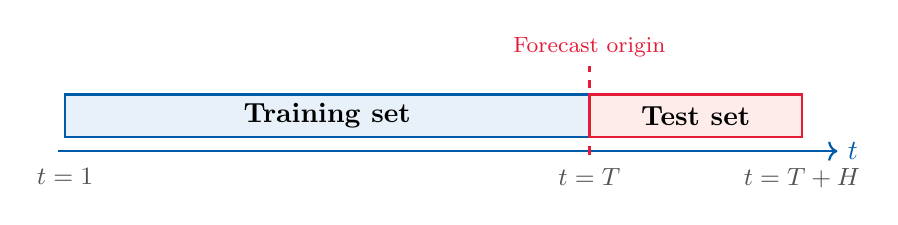
\begin{tikzpicture}[scale=0.9]
      % Timeline
      \draw[->, thick, color=unoblue] (0,0) -- (11,0) node[right] {$t$};

      % Training region
      \fill[unolightblue] (0.1, 0.2) rectangle (7.5, 0.8);
      \draw[unoblue, thick] (0.1, 0.2) rectangle (7.5, 0.8);
      \node at (3.8, 0.5) {\textbf{Training set}};
      \node[below, color=unogray, font=\small] at (0.1, -0.1) {$t=1$};
      \node[below, color=unogray, font=\small] at (7.5, -0.1) {$t=T$};

      % Test region
      \fill[unolightred] (7.5, 0.2) rectangle (10.5, 0.8);
      \draw[unored, thick] (7.5, 0.2) rectangle (10.5, 0.8);
      \node at (9.0, 0.5) {\textbf{Test set}};
      \node[below, color=unogray, font=\small] at (10.5, -0.1) {$t=T+H$};

      % Vertical dashed line
      \draw[dashed, color=unored, thick] (7.5, -0.05) -- (7.5, 1.2);
      \node[above, color=unored] at (7.5, 1.2) {\footnotesize Forecast origin};
    \end{tikzpicture}
  \end{center}
  \vspace{0.2cm}
  \begin{itemize}
    \item Model estimated on $\{y_1, \ldots, y_T\}$
    \item Forecasts $\{\hat{y}_{T+1|T}, \ldots, \hat{y}_{T+H|T}\}$ evaluated against realized values
    \item Typical test set size: \textbf{10--20\%} of the series, or a fixed future window
  \end{itemize}
  \muted{\small Walk-forward (rolling-origin) evaluation: Lecture 6.}
\end{frame}

% --- Slide: Scale-free metrics ------------------------------------------------
\begin{frame}{A Better Scale-Free Metric: MASE}
  \textcite{Hyndman2006} propose the \key{Mean Absolute Scaled Error}:
  \[
    \text{MASE} = \frac{\MAE}{\displaystyle\frac{1}{T-m}\sum_{t=m+1}^{T}|y_t - y_{t-m}|}
  \]
  \begin{itemize}
    \item Denominator: in-sample MAE of the seasonal na\"{i}ve forecast
    \item $\text{MASE} < 1$: model beats seasonal na\"{i}ve
    \item $\text{MASE} > 1$: model is \emph{worse} than the na\"{i}ve benchmark
    \item Works when $y_t = 0$ (unlike MAPE)
    \item Symmetric --- positive and negative errors treated equally
  \end{itemize}
  \vspace{0.2cm}
  \begin{keybox}
    MASE is the standard metric in the M-competitions \parencite{Makridakis2020}.
    We will use it in Lecture 6 for model comparison.
  \end{keybox}
\end{frame}

% =============================================================================
\section{Course Roadmap}
% =============================================================================

\sectionslide{Course Roadmap}{%
  What we will cover, and how it fits together.}

% --- Slide: Course structure -------------------------------------------------
\begin{frame}{BSAD 8310 in Two Parts}
  \begin{columns}[T]
    \begin{column}{0.48\textwidth}
      \textbf{Part I: Classical Econometric Forecasting}
      \begin{enumerate}
        \item \textbf{Introduction} \muted{$\leftarrow$ today}
        \item Regression-Based Forecasting
        \item Exponential Smoothing (ETS)
        \item ARIMA Models
        \item Multivariate Methods (VAR, ARIMAX)
        \item Forecast Evaluation \& Combination
      \end{enumerate}
      \vspace{0.2cm}
      \muted{\small Focus: theory + properties + principled model selection.}
    \end{column}
    \begin{column}{0.48\textwidth}
      \textbf{Part II: Predictive Analytics \& Machine Learning}
      \begin{enumerate}
        \setcounter{enumi}{6}
        \item ML Introduction \& Cross-Validation
        \item Regularization (LASSO, Ridge, Elastic Net)
        \item Tree-Based Methods (RF, XGBoost)
        \item Neural Networks \& LSTM
        \item Feature Engineering
        \item Capstone \& Applications
      \end{enumerate}
      \vspace{0.2cm}
      \muted{\small Focus: scalability, data-driven model selection, real-world pipelines.}
    \end{column}
  \end{columns}
\end{frame}

% --- Slide: Tools and expectations -------------------------------------------
\begin{frame}{Tools and Expectations}
  \begin{columns}[T]
    \begin{column}{0.48\textwidth}
      \textbf{Python throughout:}
      \begin{itemize}
        \item \texttt{statsmodels} --- ARIMA, ETS, VAR, statistical tests
        \item \texttt{scikit-learn} --- ML models, cross-validation, pipelines
        \item \texttt{pandas} --- data manipulation
        \item \texttt{matplotlib} --- visualization
        \item \texttt{numpy} --- numerical computing
      \end{itemize}
      \vspace{0.2cm}
      \textbf{Lab format:} Jupyter notebooks.
      Each lab implements the methods from the preceding lecture.
    \end{column}
    \begin{column}{0.48\textwidth}
      \textbf{What you will be able to do:}
      \begin{itemize}
        \item[\pos{$\checkmark$}] Select and justify a forecasting method for a business problem
        \item[\pos{$\checkmark$}] Implement ARIMA, ETS, LASSO, and RF models in Python
        \item[\pos{$\checkmark$}] Evaluate and compare models rigorously
        \item[\pos{$\checkmark$}] Communicate forecast uncertainty to stakeholders
        \item[\pos{$\checkmark$}] Avoid the most common forecasting mistakes
      \end{itemize}
    \end{column}
  \end{columns}
\end{frame}

% --- Slide: Key takeaways -----------------------------------------------------
\begin{frame}{Lecture 1: Key Takeaways}
  \begin{keybox}
    \small
    \begin{enumerate}
      \item Forecasting underpins every forward-looking business decision.
            Bad forecasts have measurable, costly consequences.

      \item The optimal point forecast (under squared loss) is the
            \textbf{conditional expectation}: $\hat{y}_{t+h|t} = \E[y_{t+h} \mid \mathcal{F}_t]$.

      \item Always establish \textbf{benchmark performance} first.
            A model that does not beat na\"{i}ve is not useful.

      \item \textbf{Evaluate out-of-sample only.}
            Never shuffle time series; always use \texttt{TimeSeriesSplit}.

      \item Metric choice matters: RMSE penalizes large errors;
            MAPE allows cross-series comparison; MASE benchmarks against na\"{i}ve.
    \end{enumerate}
  \end{keybox}
  \vspace{0.1cm}
  \muted{\itshape Next: Regression-Based Forecasting ---
  when and how do predictor variables improve on these benchmarks?}
\end{frame}

% --- References ---------------------------------------------------------------
\begin{frame}[allowframebreaks]{References}
  \printbibliography[heading=none]
\end{frame}

% =============================================================================
\end{document}
% =============================================================================
